\documentclass[]{report}   % List options between brackets

% List packages between braces
\usepackage[margin=1.25in]{geometry}
\usepackage{caption}              % Allows use of \caption* to omit ``Figure''
\usepackage{color}
\usepackage{tabu}                 % For tables
\usepackage{enumerate}            % List enumeration
\usepackage{float}                % Used for H placement permission to put figures in sections properly
\usepackage{graphicx}             % For rendering .eps images in document
\usepackage{listings}             % Used for syntax highlighting when including source code examples
\usepackage{titlesec}             % http://ctan.org/pkg/titlesec 
\usepackage{tikz}

% For changing the table of content entries in to hyperlinks
\usepackage[linktoc=all]{hyperref}
\hypersetup{colorlinks=true, linkcolor=blue}

% Type user-defined commands here
\renewcommand{\thesection}{}% Remove section references...
\renewcommand{\thesubsection}{\arabic{subsection}}%... from subsections

% Define custom colors
\definecolor{mygreen}{rgb}{0,0.6,0}
\definecolor{mygray}{rgb}{0.5,0.5,0.5}
\definecolor{mymauve}{rgb}{0.58,0,0.82}

% Set source code inclusion formatting
\lstset{%
  backgroundcolor=\color{white},   % choose the background color; you must add \usepackage{color} or \usepackage{xcolor}
  basicstyle=\footnotesize,        % the size of the fonts that are used for the code
  breakatwhitespace=false,         % sets if automatic breaks should only happen at whitespace
  breaklines=true,                 % sets automatic line breaking
  captionpos=b,                    % sets the caption-position to bottom
  commentstyle=\color{mygreen},    % comment style
  deletekeywords={\ldots},            % if you want to delete keywords from the given language
      %escapeinside={\%*}{*)},          % if you want to add LaTeX within your code
  extendedchars=true,              % lets you use non-ASCII characters; for 8-bits encodings only, does not work with UTF-8
  frame=single,                    % adds a frame around the code
  keepspaces=true,                 % keeps spaces in text, useful for keeping indentation of code (possibly needs columns=flexible)
  keywordstyle=\color{blue},       % keyword style
  language=Verilog,                 % the language of the code
  morekeywords={*,\ldots},            % if you want to add more keywords to the set
  numbers=left,                    % where to put the line-numbers; possible values are (none, left, right)
  numbersep=5pt,                   % how far the line-numbers are from the code
  numberstyle=\tiny\color{mygray}, % the style that is used for the line-numbers
  rulecolor=\color{black},         % if not set, the frame-color may be changed on line-breaks within not-black text (e.g. comments (green here))
  showspaces=false,                % show spaces everywhere adding particular underscores; it overrides 'showstringspaces'
  showstringspaces=false,          % underline spaces within strings only
  showtabs=false,                  % show tabs within strings adding particular underscores
  stepnumber=1,                    % the step between two line-numbers. If it's 1, each line will be numbered
  stringstyle=\color{mymauve},     % string literal style
  tabsize=2,                       % sets default tabsize to 2 spaces
title=\lstname}                   % show the filename of files included with \lstinputlisting; also try caption instead of title

\begin{document}
%\raggedright{}  % Don't allow text to be spread to the right margin

\title{Tournament Predictor}   % type title between braces
\author{Andrei Kniazev\\
  Benjamin Hunstman\\
  Michael Walton\\
  Kevin Bedrossian\\
}         % type author(s) between braces
\date{March 14, 2014}    % type date between braces
\maketitle

\begin{abstract}
  A branch predictor modeled using the Alpha 21264 microprocessor tournament predictor is simulated in software in order to demonstrate the performance of this particular technique of branch prediction.
  The predictor simply makes both a local prediction and a global prediction, and uses a choice prediction that predicts which of the two prediction techniques will be correct.
\end{abstract}

\tableofcontents

\chapter{Design}
\par{A branch predictor modeled using the Alpha 21264 microprocessor tournament predictor is simulated in software in order to demonstrate the performance of this particular technique of branch prediction.
The predictor simply makes both a local prediction and a global prediction, and uses a choice prediction that predicts which of the two prediction techniques will be correct.
Once the branch is taken or not taken we update the prediction tables as well as the path history.
The local prediction table uses a 3-bit saturation counter that is initialized to the weakly taken state.
The global prediction table uses a 2-bit saturation counter that is initialized to the weakly not taken state.}\\\\
Separate iterations of the tournament predictor were implemented, and we will briefly describe the design of both.

\begin{center}
  \begin{figure}[h]
    \label{block-diagram}
    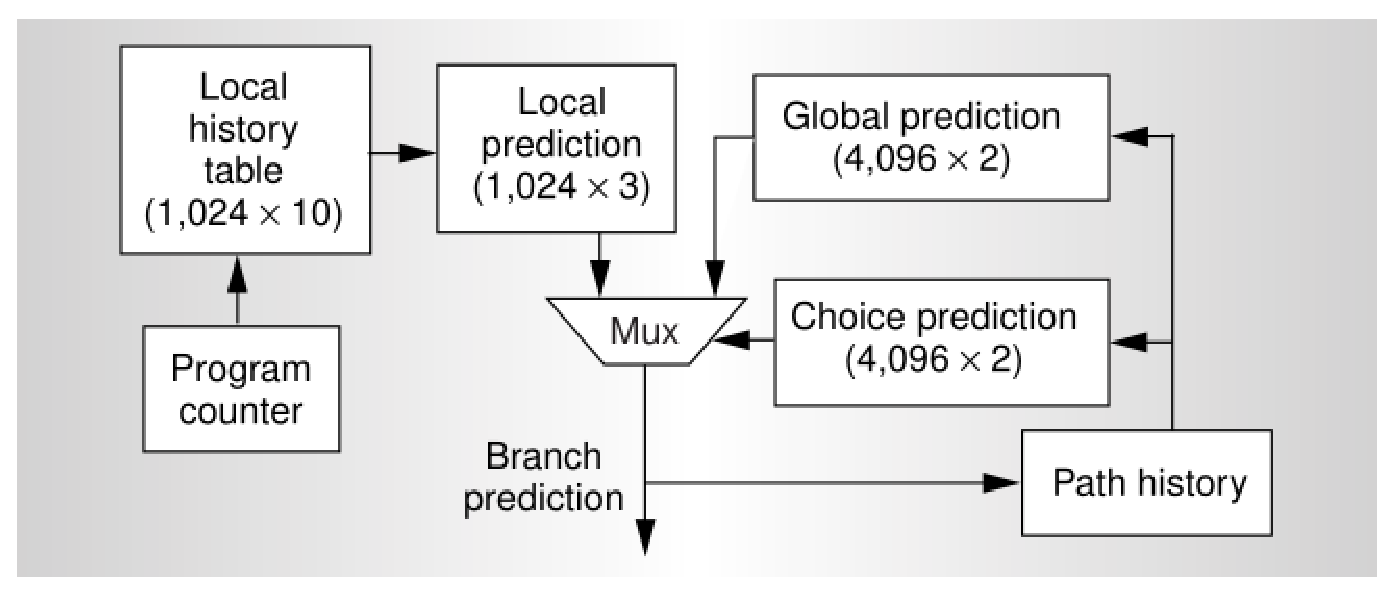
\includegraphics[width=5in]{block_diagram.eps}
    \caption*{\textit{Tournament predictor block diagram\cite{kessler}}}
  \end{figure}
\end{center}
\pagebreak

\section{Implementation 1}
\par{Since the branch prediction appeared to be built around seperate width saturation counters we develop a class called saturating counter.
It would be able to be an arbitrary width using parameters for the constructor.
This allowed us to test the saturating counter methods completely independent of the predictor framework.
We built a small main function that created saturation counters of varying width, and incremented/decremented the counters in a test loop.
Once this was completed all the predictor class needed to do was create dynamically allocated arrays of the counters with the proper widths.
The makefile was slightly modified to include the extra source files as well.}

\section{Implementation 2}
Talk about Ben's implementation of the tournament predictor

\begin{center}
  \begin{figure}[h]
    \label{state-machine}
    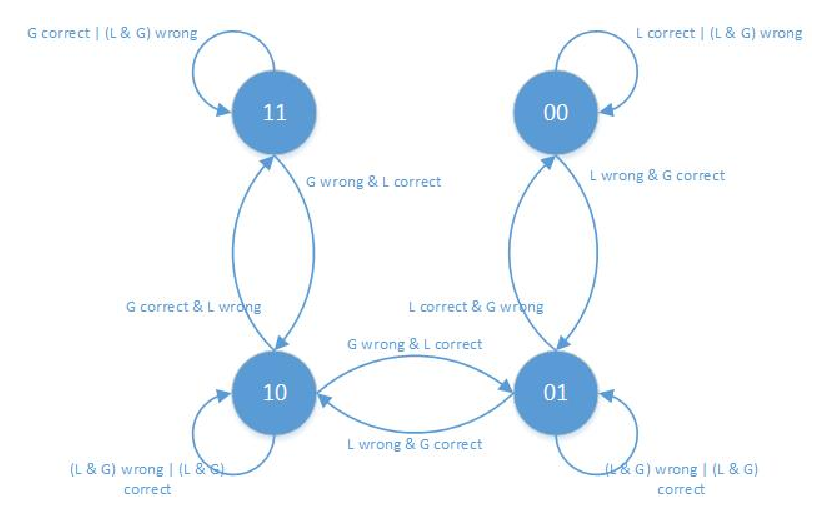
\includegraphics[width=5in]{CPT_FSM.eps}
    \caption*{\textit{Finite-state machine of tournament predictor}}
  \end{figure}
\end{center}

\chapter{Testing}
\par{This chapter describes validation of the tournament predictor.
Initialization values of the saturation counters and path history are described as well as test methods.
Both implementations will be discussed separately for what's necessary.
Our own framework was developed in order to control debug information being printed as well as to produce trace files containing the information in each branch as well as whether our tournament predictor had predicted taken or not taken.
Results from both implementations using a common trace file via the custom framework were the same.
In order to verify using the trace file we disabled local history update in order to make changes in the choice \& global tables immediately observable.}

\section{Implementation 1}
\par{Validation began with verification of the saturation counters.
As described in the design the testing was simply to observe proper values in the counter.
Next was to validate that each predictor was working correctly; for this we created tests that would target (or favor) a particular predictor.
This way we could coerce a predictor all the way to the saturation point using a long string of consecutive taken or not taken values.
The global predictor was more challenging because we needed to use a pattern that the local predictor would mispredict.
The answer to testing the global predictor was to use a pattern of taken/not taken in alternation.}
\par{How the path history was changing was also taken in to account during debugging of the global predictor in order to verify correct predictions of the global predictor.
Having the path history printed out during debugging was helpful for debugging the choice predictor as well.
Testing the choice predictor consisted of switching between using the tests for the local and global predictors.
Due to the nature of these tests we would also be able to observe the choice predictor tending toward the predictor that was correct.
Since these test cases were designed to isolate local or global the choice prediction would follow naturally if implemented correctly.}

\section{Implementation 2}

\subsection{Testing Initialization}
Several initialization values for the saturation counters were considered, and the following is the resulting benchmarks for each initialization value:

\begin{center}
  \begin{tabular} { c c c | c c c || c }
    Local & Global & Choice & FP & INT & MM & Notes\\
    \hline
    0 & 0 & 0 & 4.668 & 12.795 & 9.323 & Strongly not taken/Strongly Local\\
    3 & 1 & 0 & 4.664 & 12.774 & 9.325 & Weakly not taken/Weakly Local\\
    3 & 1 & 1 & 4.332 & 9.589 & 8.858 & Weakly not taken/Weakly Local\\
    4 & 1 & 1 & 4.287 & 9.877 & 9.002 & Weakly not taken/Weakly Local\\
    4 & 2 & 0 & 4.630 & 12.662 & 9.193 & Weakly taken/Strongly Local\\
    \#4 & 2 & 1 & 4.287 & 8.765 & 8.767 & Weakly taken/Weakly Local\\
    4 & 2 & 2 & 4.297 & 8.722 & 8.796 & Weakly taken/Weakly Global\\
    4 & 2 & 3 & 4.297 & 8.721 & 8.809 & Weakly taken/Strongly Global\\
    7 & 3 & 3 & 4.318 & 8.741 & 8.834 & Strongly taken/Strongly Global\\
  \end{tabular}
\end{center}
\# represents chosen initialization

\subsection{Test functionality of each predictor}
\subsubsection{Local Prediction Table}

\begin{itemize}
  \item{Verify that LPT stays in predict taken state by giving it multiple branches that will test each direction of the counter of the taken side. Actual outcome of branches will be TTTTNNNTTT. Predicted outcome was <insert from spreadsheet>. Note: first branches tests that it goes to strongly taken; next three test to see that it goes back to weakly taken.}

  \item{Test that it switches from taken to not-taken by giving it multiple branches that
    are first taken then not taken and back again to check both directions. Actual outcome of branches will be NNTTTNNNN. Predicted outcome was <insert from spreadsheet>. Note multiple branches go to the same saturation counter. This is not really ideal but is necessary due to constraints.}
\end{itemize}

\subsubsection{Global Prediction Table}
The path history must be preloaded to ensure it goes to the same sat counter each time.

\begin{enumerate}
  \item{Test that it stays not taken by giving it multiple branches that are all actually not taken.}

    \begin{itemize}
      \item{The pattern needed for preloading the path history to ensure use of the same counter will be to just use 0 every time it goes through}
      \item{Pattern for actual branch outcome will be NTNNTNNTNN. Predicted output was <insert from spreadsheet>.}
    \end{itemize}
  \item{Test that it switches from not-taken to taken by giving it multiple branches that are first not-taken and then taken.}
    \begin{itemize}
      \item{Pattern for preloading path history is the same as above. Predicted output was <insert from spreadsheet>.}
      \item{Pattern for actual branch outcome will be NTTTNNTNTT. Predicted output was <insert from spreadsheet>.}
    \end{itemize}
\end{enumerate}

\subsubsection{Choice Prediction Table}
The path history must be preloaded to ensure it goes to the same saturation counter each time.
\begin{enumerate}
  \item{Test that it stays local by giving it multiple branches that local would be correct in its prediction and then switch to global.}
    \begin{itemize}
      \item{Pattern for actual branch outcome is NNNNNNTTTTTT. Predicted output was <insert from spreadsheet>.}
    \end{itemize}
  \item{Test that it switches from local to global by giving it multiple branches that would cause it to switch back and forth between predictors}
    \begin{itemize}
      \item{Pattern for actual branch outcome is NNNNTT. Predicted output was <insert from spreadsheet>.}
    \end{itemize}
\end{enumerate}

Note: the first 4 are not taken so that it will put both L and G predictors to strongly not taken, but because it only takes two incorrect branches for the global predictor to switch to taken it is possible to get the global predictor to predict correctly before the local predictor.


\chapter{Source Code}
\section{main.cc}
\lstinputlisting{../src/main.cc}
\pagebreak

\section{Implementation 1 predictor.cc}
\lstinputlisting{../src/AKs/predictor.cc}
\pagebreak

\section{Implementation 2 predictor.cc}
\lstinputlisting{../src/Ben's/predictor.cc}
\pagebreak

\bibliographystyle{plain}
\bibliography{kessler}
\end{document}
